% The compilation pipeline, as the roadmap for the "How anvl works" part.
\documentclass[tikz, border=10pt]{standalone}
\usetikzlibrary{arrows.meta, positioning}

\begin{document}
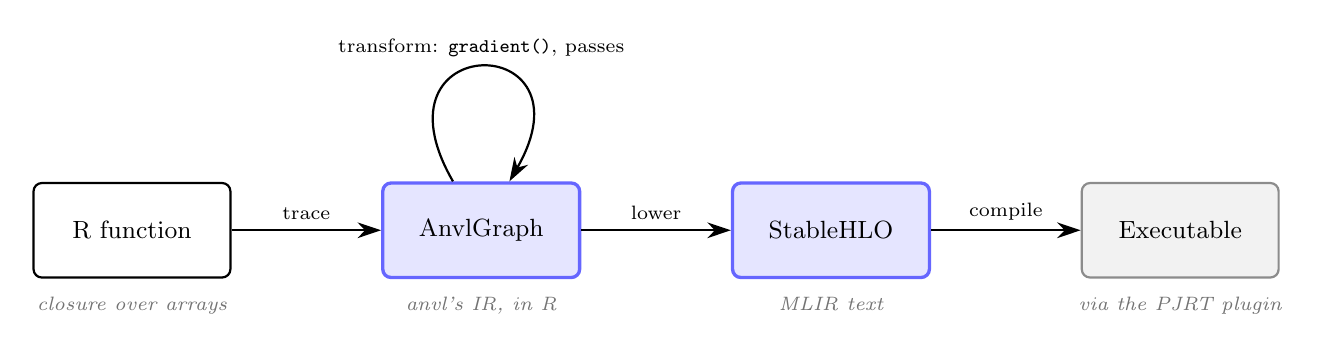
\begin{tikzpicture}[
  node distance=1.9cm,
  box/.style={
    draw, rounded corners=3pt, thick,
    minimum width=2.5cm, minimum height=1.2cm,
    align=center, font=\small
  },
  ir/.style={box, fill=blue!10, draw=blue!60, very thick},
  ext/.style={box, fill=black!5, draw=black!45},
  arr/.style={-{Stealth[length=3mm, width=2mm]}, thick},
  lab/.style={font=\scriptsize},
  note/.style={font=\scriptsize\itshape, text=black!55, below=3pt}
]
  \node[box] (R) {R function};
  \node[ir, right=of R] (G) {AnvlGraph};
  \node[ir, right=of G] (S) {StableHLO};
  \node[ext, right=of S] (E) {Executable};

  \draw[arr] (R) -- node[above, lab] {trace} (G);
  \draw[arr] (G) -- node[above, lab] {lower} (S);
  \draw[arr] (S) -- node[above, lab] {compile} (E);
  \draw[arr] (G) edge [loop above, looseness=8, out=120, in=60]
    node[above, lab] {transform: \texttt{gradient()}, passes} (G);

  \node[note] at (R.south) {closure over arrays};
  \node[note] at (G.south) {anvl's IR, in R};
  \node[note] at (S.south) {MLIR text};
  \node[note] at (E.south) {via the PJRT plugin};
\end{tikzpicture}
\end{document}
